\section{Ship of State}

\begin{quotex}
Propaganda must become as natural as air or food. It must proceed by psychological inhibition and the least possible shock. The individual is then able to declare in all honesty that no such thing as propaganda exists. In fact, however, he has been so absorbed by it that he is literally no longer able to see the truth. The natures of man and propaganda have become so inextricably mixed that everything depends not on choice or on free will, but on reflex and myth. The prolonged and hypnotic repetition of the same complex of ideas, the same images, and the same rumors condition man for the assimilation of his nature to propaganda. \flright{\textsc{Jacques Ellul}}

Those who fail to govern risk being governed by their inferiors. \flright{\textsc{Plato}, \emph{The Republic}}

\end{quotex}
In the \emph{Republic}, \textbf{Socrates} compares the democratic system to a ship. The shipowner needs his ship to reach a destination. All the sailors quarrel among each other, all claiming to know how to navigate the ship safely. They even resort to currying favor with the owner. Meanwhile, the navigator, who gets his skill from gazing at the stars and is therefore the only one who really knows how to direct the ship, is ignored.

\paragraph{Physiognomy}
\textbf{Julius Evola} believed that physiognomy, the study of the meaning of the human face, has an important role in the study of race: not biological race, but rather as a window into the race of the soul. In its crude form, physiognomy is a pseudoscience since it claims to determine permanent character traits from static facial features.

However, by observing facial features dynamically, they give a clue to the inner soul life of a person; this is one aspect of the Hermetic teaching on ``external considering" (see Note). Evola includes an Appendix to his \emph{Summary of the Doctrine of Race} which includes photographs of different types. Rather than posed pictures, he would have preferred photos taken during ``one of those moments in which the deepest and most expressive elements" are revealed. Keep in mind that 80 years ago, photos were hard to come by and certainly were not as easily accessible as they are now.

There is some actual science behind this. Although there are about 43 muscles in the face, only 5 are necessary to express the six universal facial expressions: happiness, sadness, fear, anger, surprise, disgust. However, the remaining ``assisting muscles" actually add the personal character to the facial expression. That is why training is required for actors. Consciously making those basic expression looks artificial and forced; that is why, for example, people can see through a fake smile. However, controlling all those other muscles is not easy. In method acting, which study I would recommend to Hermetists, the actor tries to recall a personal incident, analogous to the role he is playing, in order to relive it. In that way, the facial expression should be more natural and expressive.

NOTE: Besides facial expression, careful observation of posture, nervous movements, voice intonations, etc., are used to become attuned to another's inner state. Beyond that, the responses to certain probing questions may be taken into consideration.

\paragraph{Identifying Caste Membership}
One of the traditional teachings is that few of us are in our natural castes in this age. Evola had this to say about the selection of his photographic material:

\begin{quotex}
The great part of the photographic material is affected by a democratic prejudice: in most cases, they are photos of people of the lower or middle classes. While it would be more important and interesting to consider the highest exponents of a people: its nobility, military and political leaders, priests, and intellectuals. 

\end{quotex}
Although it takes some practice to become skilled in the art and science of physiognomy, it may be worthwhile to practice with available images. Specifically, take a look at the leaders of a nation, or a political party, or an intellectual movement, even the priests or religious leaders? Do they reflect nobility or a sense of transcendence? What do they reveal about the people who accept them? Of course, in our democratic age, the populace will gravitate towards those who look most like them.

\paragraph{The Purpose of Political Parties}
In the USA, which is dominated by two parties, people complain about the lack of choice. In other nations, too many parties prevent governance. Suppose political parties actually stood for something. For example, a party would be committed to a particular and well-articulated intellectual tradition. Its leaders would be trained in that tradition. Office seekers would be vetted by the party before being allowed to run for a political office. That might include health records, psychological profiles, IQ or aptitude test scores, and so on. Or on the other hand, we could just keep the Ship of Fools going as is as long as possible.

That is probably not possible in a democracy. However, the situation in Tradition is different; it is similar as far as intellectual integrity goes, but there is no need for multiple parties. For Tradition, according to \textbf{Rene Guenon}, the spiritual leaders follow an unbroken chain and the originary spiritual impulse is passed down from generation to generation.

Similarly, the political class was based on an aristocracy of merit that embodied the highest and noblest ideals of a people.

Perhaps the many alternative movements around today could follow this pattern. They would follow a consistent philosophical, scientific, metaphysical, or political tradition. Its leaders would have to demonstrate competence in that tradition. They would post photographs exhibiting their noble bearing, as well as their qualifications. \emph{We need to identify the stargazer, not the sailors}.

\paragraph{Polish Thought Police}
\begin{quotex}
Once upon a time, at a conference of Evangelical theologians, a small group went out to dinner at a nice restaurant. The pretty waitress came to the table and asked, ``Would you gentlemen like a cocktail first?" The theologians looked at each other awkwardly until one of them finally spoke up. ``Uhh," he said, ``we don't drink … at least not in front of each other." 

\end{quotex}
Years ago, I had the pleasure of knowing a Polish gentleman, a physicist, who had gotten onto a train to Austria without money or possession, disembarked in Vienna, and sought asylum. Over bottles of vodka, we would discuss life behind the Iron Curtain.

The most difficult thing was the pretense. By the late 1970s, the illusion of Marxism could no longer be maintained. Nevertheless, in a university setting, no one wanted to be the first to speak up for fear of the possible repercussions. Hence, for show, they would study Marx and shout, ``Power to the People".

Paradoxically, that seems to be the situation in the West. If you are among those who are convinced that 2+2=5, then you feel no discomfort. Otherwise, you do.

\paragraph{Gaslighting and the Authoritarian Personality}
Gaslighting is a form of mental abuse in which a sociopath, for example, tries to convince the victim that he is insane. We see that at work in political discourse. Vague accusations of racism, homophobia, misogyny, and so on, are made willy-nilly, in order to impugn the mental stability of candidates or their supporters. Attitudes that well-bred men used to believe were healthy and normal—from the big bang to a couple of generations ago—are not anathematized. That is the price of progress.

A prime example of this is a recent study on the so-called ``authoritarian personality" (which I saw on GPS this weekend). Now the original study was made some 70 years ago by the Frankfurt School, allegedly to identify potential fascists. The new study is even worse.

The professor claimed that the identifying mark is the desire for ``Law and Order". Now I don't like these interview shows because the interrogators are seldom intelligent or quick-witted enough to ask the correct follow up questions. The alternative is illegality and disorder, isn't it? That sounds absurd on its face, until you think it through and see that it is actually endemic to the modern world. The overlooking of the illegal and the use of disorder as a political tactic is abundantly clear.

Unfortunately for his case, the real authoritarian personality is not the one in favor of law and order. Under the rule of law (at least in its ideal), justice is blind and does not depend on the arbitrary whim of a ``strong man". The opposite case, however, can only be resolved by the strong man. For example, a while back Chris Rock compared the President and First Lady as the mom and dad of a country who should be obeyed.


\hfill

If so interested, I will allow photo comparisons in the comments. As an example, compare the photos of Pope Francis to Pope Pius XII.

\begin{figure}[ht]
\centering
\begin{minipage}{.45\textwidth}

\includegraphics[scale=.5]{a20160315ShipofState-img001.png}
\end{minipage}~%
\begin{minipage}{.45\textwidth}
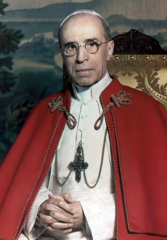
\includegraphics[scale=.5]{a20160315ShipofState-img002.png}
\end{minipage}
\caption{Pope Francis / Pope Pius XII}
\end{figure}

\hfill



\flrightit{Posted on 2016-03-15 by Cologero }

\begin{center}* * *\end{center}

\begin{footnotesize}\begin{sffamily}



\texttt{Cologero on 2016-03-18 at 12:29 said: }

Here are some examples of the use of lawlessness and chaos as a political tactic.

\textit{When the Law Is a Drag:} \url{https://pjmedia.com/victordavishanson/law-is-a-drag/?singlepage=true}

\textit{France's Highways Descend Into Chaos \& Lawlessness:} \url{http://www.zerohedge.com/news/2016-01-26/frances-highways-descend-chaos-lawlessness}


\hfill

\texttt{Sparrow on 2016-03-21 at 00:15 said: }

Coincidentally, I've recently been reading on Hegel's views of the spirit and physiognomy. Racial political correctness did not exist back in the day, but Hegel seems quite eager to correct himself. He asserts that ``spirit leaves nothing to chance," then in another work asserts that physical differences do not reflect the spirit and are ``accidents." of course, the physiognomy of Hegel's day was largely materialistic, he may have been more accepting to Evola's belief in spiritual races.


\hfill

\texttt{Olavsson on 2016-03-21 at 14:37 said: }

We could compare Julius Evola and Frithjof Schuon, two ``Traditionalists" with a widely different style. Video is even more useful than photographs, as we can study changing expressions, voice intonations, gestures etc in better detail.

Schuon:

\url{https://www.youtube.com/watch?v=F9T90GWfk40}

Evola:

\url{https://www.youtube.com/watch?v=QiCtdi5nCoA}

Note that both men are aging in these recordings, so we see them after they have matured as much as they were capable of.

Evola comes much more alive to you when watching him in this format, than when seeing a few old black-and-white photographs for which he had posed pretentiously. He's certainly got charisma. Every now and then he reveals something almost ``vampyric" in a romantic-draculian-aristocratic sense (which I suspect he would even have taken as a compliment). It is also easy to see that he still retains strong residues of attachment to the ego-self. Does he come across as `noble'. Definitely, but mainly in the cultural and human degree of appealing to a historical archetype, which is done deliberately and self-consciously. I accept Evola's own discernment that he was a kshatriya as far as this four-fold caste-categorization is concerned. The entire aura of Schuon, on the other hand, is very characteristic of the sagely type, which is `noble' (arya) in a higher octave altogether. He appears spiritual in a deeper, more essential and selfless sense. (Note that I'm here ignoring the various personal controversies and so on, which would be to stray from the context in question.) But both men, Schuon as much as Evola, were possibly too concerned with outer image, and even in the case of Schuon, this might be a sign of a sublimated vanity. The purest spiritual nobility is that of men who do not deliberately and self-consciously act or appear in a certain manner because they know this is what signals nobility or spirituality, but rather that of men who spontaneously be this way without any thought of the self or any desire thereof or self-interest, who are genuinely selfless before the Divine as well as before others, and thus let the Heavenly wu-wei flow through them unhindered.

For we whose foremost interest when it comes to these men is the validity of Traditional doctrines and truths, the question of their personal qualities aside from their intellectual ability to get these things straight (and none of them—especially not Evola—were entirely infallible or unbiased in this respect) is largely uninteresting. But in this context, when we're concerned with the personal dimension, it may hold some limited relevance. In the preface to the English edition of `Introduction to Magic' (page xiv), we see that Evola's ex-lover Sibilla Aleramo says of him: ``He is inhuman, an icy architect of acrobatic theories, vain, vicious, perverse…" To Evola's defense, it may be pointed out that she was hardly unbiased, and her experience was with the young `magical' incarnation of him.

It should always be remembered that ``not all that is gold will glitter" when we study these things. A man or woman of high spiritual stature, or nobility, may not necessarily give us that impression immediately based on more superficial factors, our prejudices, preconceptions and so on, as our eye—and our integral knowledge—is simply not sufficiently subtle to notice everything that transcends our own inner condition to a considerable extent, and which may be concealed from curious eyes. But these things are never impossible to see for those possessing the required knowledge, as they leave definite signs in the outer being: whether WE as individuals, given our own limitations, are able to consciously register it is quite another question. Also, as the Christ said according to the Gospel of Thomas, ``There is light within a person of light, and it shines on the whole world; if it does not shine, it is dark."

One thing I do notice these days is that the outright evil of many members of the modern `elites' is very clearly reflected—in fact often grossly visible—in their countenance, almost as if they were demonically possessed. Especially the eyes are usually very revealing in this respect, being the ``mirror of the soul". There are many, many examples one could refer to, but in these days, Hillary Clinton would be one appropriate case to mention. For those who have eyes to see, the agents of the dark-side may be quickly identified thus, and one may even derive from such observation an impression of the varying degrees of inner `demonization' (being the fall into the infra-human, as Guenon would say, almost as an inverted transcendence) that dominate different personalities. Here we are dealing not merely with cases of inept and incompetent, mediocre `plebeians' who have been able to ascend to the ranks of power because of the quantitative reign of `demotism'. but in fact with something far more sinister. We must realize that there are even highly ``intelligent" and cunning elitists who work under the sign of evil, who are more than what the official images and stories that are presented make us believe. Without being able to see into the depths of such figures, to see which principal forces (and intelligences) they are serving and are infiltrated by (``possessed" of) beyond/behind the official political and ideological facade of the most superficial interests and agendas, we will remain forever blind to what Evola termed ``the third dimension of history" in his commentaries on the ``occult war."

Some final words: For the highest norm of a noble inner as well as outer ``style", we can do no better than studying sages and masters, saints etc whose lives were wholeheartedly dedicated to a single-minded quest for Divine Truth. To the extent they are fully permeated by this path, and have integrated their insights fully, it will show. No person should be taken as an ideal embodiment of any kind unless they are truly holy. Then it will only be a matter of the ``blind leading the blind." But if we mimic them for the sake of our egos, instead of sacrificing ourselves fully to the Way, we will have missed the entire point.


\hfill

\texttt{Harun on 2016-03-22 at 04:44 said: }

I would also consider a few legends about people looking the same.

The state of the being of someone can influence his physical appearance.

For example is the count of St.Germain immortal or is he a succession of initiates that look very similar and also share memories?

Also, Guénon mentioned in a letter to De Giorgio that St.Pius of Petralcina looked very similar to a contemporary sufi sheyk.


\hfill

\texttt{Cologero on 2016-03-22 at 21:19 said: }

Although the saying goes ``never judge a book by its cover", people can't avoid it. Of course, any worthwhile physiognamy isn't interested just in physical attractiveness. Presumably Evola, growing up in Italy, would have been aware of the tradition of physiognamy described in the following links (not taught in RCIA classes AFAIK):

\textit{The Eyes and the Gaze:} \url{http://www.traditioninaction.org/Cultural/A018cpManualCivility6_Gaze.htm}

\textit{The Face Reveals the Heart of the Man:} \url{http://www.traditioninaction.org/religious/n001rpFaceRevealsMan.htm}

\textit{Four Ways to Discern a Man's Soul by His Appearance:} \url{http://www.traditioninaction.org/religious/n003rpLapide_Appearance_2.htm}

\textit{The Eyes Are the Mirror of the Soul: } \url{http://www.traditioninaction.org/religious/n002rpLapide_Appearance.htm}


\hfill

\texttt{Cologero on 2016-03-22 at 21:40 said: }

Many interesting points, Olavsson. I would just confirm that the ordinary person is quite unskilled in this science, otherwise con men and psychopaths, not to mention most politicians, would have no careers. I recall my time at voir dire for jury selection. The attorney asked each of us how could we tell if someone was lying. Most women asserted they ``could see it in their eyes". I'm sure that outside the courtroom, those very women would complain about all the lies that men had told them.

Vanity traditionally has been considered the most subtle vice, since it often follows great spiritual progress. It seems unavoidable for anyone who strives to be a public figure, since motives can easily be confounded.

As for Miss Aleramo, her reaction is likely due to Evola's transcendence of bourgeois values. In particular, women sometimes get upset when a man can't be manipulated sexually.


\hfill

\texttt{Boreas on 2016-03-23 at 08:28 said: }

Interesting points Olavsson regarding Evola and Schuon. I've come to think Evola as some sort of a LHP figure lately, and this `personal equation' that he himself talked alot could perhaps show out also in his facial expressions and gestures. In my opinion there was always something `luciferian' about Evola, and this would show up both in his actions, in his personal weltanschauung and even in his physical personality. He was more a ``soulful" personality than purely ``spiritual" as for example Guénon or Schuon.

This also reminds me of Guénon's view that the ``revolt of the Kshatriyas" was a `luciferian' phenomenon (he mentioned it in `Spiritual Authority and Temporal Power'. if I recall correctly).


\hfill

\texttt{Max on 2016-03-29 at 09:08 said: }

Most people have quite boring facial features and expressions. Evola has an idiosyncratic expression as one would expect. One can usually come into contact with interesting people by simply being on the look out for interesting and differentiated expression. The predominant emotional state of a person often shows in the face, and there are often many signs of negative emotion in various forms. 

When studying people in for example public transport, it is very unusual to see someone who seems to be inner motivated – most are being carried away by various stimuli and acts as if on auto-pilot. Nowadays it is very rare to see someone simply sitting straight up with a good posture, having a clear and awake gaze, not distracting himself with some gadget, slumbering, talking loudly and incoherently, or just plain mentally drifting. The other day I was on the commuter train and an elderly couple clearly on temporary visit sat down on the opposing seats, actively seeking my eyes and smiling, there was a sense of emphatic and polite understanding, like a refreshing flash from a world that does not exist anymore, it made me think of what we have lost.


\hfill

\texttt{Olavsson on 2016-04-02 at 15:16 said: }

@Alistair Fraser:

There is an idea in certain initiatic currents that a highly capable master may, under certain conditions, ``transmit" by his power a particular inner state into a qualified disciple, an awakening to a higher state inspired by that direct contact with one in whom the inner state is transcendent in relation to one's own. In other words, an act of spiritual grace using the master as an intermediary. This may be very distantly related to what you experienced with that woman, though on a far more ordinary level. Of course, I think it's quite normal to have at least a small awareness of how differently we may be affected by the contact with diverse human types. It is important to learn the art of analyzing the effect of these contacts from the viewpoint of spiritual priorities. For example, we can decide to ``ride the tiger" of Kali-yuga and hang out at decadent underground nightclubs in the cities and risk being affected by the negative influences at work in such places, or we can simply stay away and distance ourselves increasingly from the low spirit of the times, thus creating ideal conditions for the contemplative path. (Beata solitudo, sola beatitudo…) We've always got a choice.

The same goes for the insidious onslaught of subversive propaganda that you mention, by which we are ambushed from all directions nowadays. We must close our doors upon it to the exact extent this is possible given our circumstances. Regarding propaganda (mentioned in Cologero's post), I recently came across an intriguing satanic counter-initiate (founder of the Temple of Set) who used to work within US military with an above top secret security clearance, Dr. Michael Aquino; he has apparently written a book called `MindWar'. regarding which he says:

``There is no defense whatever against MW PSYCONs, because they access the subconscious, not the conscious thought process. You would have absolutely no idea a MW campaign was being directed against you unless you knew exactly what to look for, and quite possibly not even then."

But if we are firmly rooted in an orthodox Traditional worldview, metaphysics and esoterism, and are able to thoroughly and deeply apply the proper First Principles to everything, always remaining watchful and guarding our own minds, I cannot see how exactly the enemy would be able to influence us through the subconscious to the degree of conditioning our reactions and orientations in the world. There is a great difference between the average man in the street and, say, a Guénon. So why does our satanic Dr. Aquino want us to believe there is ``no defense whatever" against it? Curious, isn't it? Perhaps in order to subtly plant the sinister suggestion that certain elites are almighty, like God, and cannot possibly be opposed? Men like him, and so much the more when they have been involved in extensive scientific research into these matters, are masters of manipulation, and everything they say should be closely scrutinized, never taken at face value.

Re: the Evola video footage: It is true that this interview was filmed after his war accident, but his entire upper body was unaffected, so I don't think his facial expressions and so on would have been particularly changed. He seems pretty natural and effortless in that video. I would have paid more to see a video of Guenon than the younger Evola, as a matter of fact. Also, being more or less Hermetists, after all, we will know that this very significant and dramatic incident in the life of Evola symbolically corresponds to a facet of his inner condition. Evola himself—having a metaphysical and spiritual rather than profane/modern outlook on every aspect of reality—knew it wasn't a mere isolated coincidence, but he apparently never attained certainty as to the deeper reason for his fate. If my memory serves me right, Mircea Eliade also thought it signalled something about his inner condition. My own suggestion is that the answer to why it happened was hidden where Evola would have been the least interested in searching for it, as it would (perhaps) have humbled him more than a little. Anyhow, he faced these challenging last years of his life with admirable inner strength, and I hope that God granted him in death at least some of the liberation he had lived for. How interesting it would have been to be able to trace his (and others'. postmortem destiny.

@Cologero:

Seeing through lies is not so easy if one wants to believe the lies. One word: detachment. And what you say about vanity is the plain truth.

Re: Aleramo: You might be right about that. While I am as defiant towards the bourgeois way of life as anyone, simply because it is completely contrary to my nature, one should nevertheless be careful not to make this a guiding principle of its own, which may possibly even take precedence over more essential principles. What must ultimately be transcended is the lower self, after all, which is perfectly capable of reinforcing itself even while `transcending' bourgois norms.

@Boreas:

You are right to view Evola's own chosen course as basically ``LHP" (``Left-Hand Path), which I do not think he would have protested, based on various statements in the video interview I linked to, for example. Here we can mention his individualistic and independent approach to the path, not having made commitment to any formal tradition, but that is widespread in our age and doesn't necessarily make one LHP. However, his insistence on not answering to any spiritual authority higher than his own individual self, almost a `promethean' approach to transcendence (which is why the way of the magus initially appealed to him), his fascination with what he himself termed the ``antinomianism" of certain Hindu tantras (a tradition which Guénon, incidentally, thought Evola wasn't fit to deal with…), and his attempt to practice Left-Hand Tantrism as a `freelancer' outside a proper traditional context—all of this, and more, combine to make him quite LHP, if we define this term in the broadest fashion possible, allowing for many nuances. It is important to emphasize, however, that this does not at all mean he considered his own solution an ideal path to be emulated from a general point of view. (For example, he referred someone to Sufism, curiously saying that he himself was more interested in ``power" than spirituality.) Personally, I am prone to suggest that Evola placed spiritual limitations upon himself, ironically due to a quest for individual spiritual freedom, independence and self-sufficiency, that could have been overcome if he had submitted himself to a more regular path as was done by a Guénon.

As for Evola's ``personal equation", I think you are right in describing him as more of a ``soulful" than a ``purely spiritual" type, which is not so strange considering his kshatriya nature. He often spoke of the unconditioned Absolute, but due to this personality factor, I doubt that he would ever have been suited for anything above the ``Lesser Mysteries", which in any case is the initiatic domain that has typically been appropriate for kshatriyas according to Guénon. Esoterism in Europe seems seldom to have went beyond it.

And speaking of the ``revolt of the kshatriyas", it is interesting that Red is considered a stage superior to White in esoteric alchemy, which (as Evola never tired of pointing out) identifies itself much with royal symbolism—almost as if the Will is above Intellection, or the Soul above the Spirit. This is a theme that keeps returning in deviated initiations. (Well exemplified by Crowley's famous maxim, ``Do what thou wilt shall be the whole of the law", as if the Great Quest can start and end with the isolated self-will of some individuated ``I" that is, moreover, in a fallen state).

Also, there are several things that could be mentioned in connection to the ``revolt of the kshatriyas", Luciferianism and the Counter-Initiation, all of which may be inter-related, but it will have to wait, for this comment is getting too lengthy.


\hfill

\texttt{Tom on 2016-04-07 at 05:47 said: }

There are examples in Indo-European traditions of Physiognomy besides the obvious caste distinctions of Hinduism. In Old Norse literature we can see clearly from Rígsthula that the three castes could be identified by physical characteristics with the lowest being the darkest. More subtle examples can be found in the sagas where physical attributes have cultural and symbolic significance in. They reveal aspects of a person's character, disposition and their future. Very often the symbolic nature of a character is identified by their lineage and their behaviour, but both of these variables can in turn be related to the physical attributes of that character. In Njals saga, Hrútr describes his niece Hallgerdhr as having ``thieves' eyes", which is a portent to the coming events of the novel generated by Hallgerdhr's un womanly and dominating nature. later in the saga Hallgerdhr makes scathing comments about the appearances of Bergthóra, Njáll, and their sons (whom she calls dung-beardlings due to the implied shame of the fact their father Njall is unable to grow a proper beard); this physical lack is a signifier of implied sexual inadequacy. All this contrasts greatly with the physical description in the same saga of the heroic character Gunnar:

``He was handsome and fair of skin and had a straight nose, turned up at its tip. He was blue-eyed and keen eyed and ruddy cheeked, with thick hair, blonde and well combed."


\hfill

\texttt{Thomas Blanchard on 2016-07-11 at 16:49 said: }

I was reminded of this post while reading Plinio Corrêa de Oliveira's physiognomic analysis of political revolutionaries' faces, which I'll share here as it may be of some interest: \url{http://nobility.org/2016/02/18/three-faces-of-the-revolution/}

As children, it feels natural to make inferences about character based on physical appearance (and particularly facial features), although most modern adults suppress these judgements as they're taught not to.


\hfill

\texttt{Max on 2016-09-11 at 14:56 said: }

Here is a passage from George Duby's book on medieval artwork ``The Age of the Cathedrals" under the heading of ``Faces":

``The growing number of characters in the liturgical drama filling the theaters in the cathedral porches meant that each had to be distinguished. Certainly they bore their insignia, the special attribute given to each prophet, each precursor, each apostle in Christian iconography, but they also had to be endowed with personal features capable of conveying a specific psychological expression. The vocabulary of the literary works available to knights in the thirteenth century was extremely poor. Joinville abounded in eloquent portrayals of spirited combat and the motley glamor of courtly gatherings, but became tongue-tied when it was a matter of describing character. In practical life at any rate, in the surveys carried out to ascertain the distribution of feudal rights or to settle points of usage and sometimes even before their confessors, the lords, great and small, gradually sharpened their analytical ability. As for the academic world, it was accustomed to introspection, which already offered a foothold for the morality of Abelard. All theology led to ethics. It involved the exploration of the soul, the classification of its capacities and its virtues. And as the intellectual system of doctors was based on the principle of the unity of the universe, as it asserted the close cohesion of the three components of the human being – mind, soul, and body – it naturally considered that facial features faithfully translated individual dispositions. The scholastic approach, however, was bent on resolving the particularities of each individual through the forms common to his species. It proceeded by distinguishing kinds. More exactly, then, the faces of the statues represent types of men."

The practical science of Physiognomy then, seems primarily to have been a domain of artisans and knights rather than schoolmen, which contributes to its perception as a Hermetic discipline, for in the old tales we find the wise hermit as a retired knight. The intellectual class can be prone to too much abstraction when focusing at what is common to the species, which we need to remember is nevertheless made up of individuals with distinguishing marks. The usage of ``species" seems to have undergone quite a lot of change throughout history and should refer more to what is ``seen" as a ``medium of knowledge" than a dry external classification. \url{http://www.newadvent.org/cathen/14210a.htm}

On the topic of seeing I found the man in this photo an interesting study, perhaps with a tangent to Swedenborg's claims on hidden teachings, which is unlikely to refer to physical writings in any case: \url{http://frontierphotos.blogspot.se/2008/11/bonpo-lama-from-radja-gomba.html}

Primary importance is given to the subtle expression rather than hard facial features, even though those matter as well. This poses a difficulty for art and sculpture since it is naturally easier to capture the outward form than the formless aspect of a person. However, in the ancient world they would also ritually ``animate" statues so as to not merely see it as a lump of rock. 

The species cannot, in the manner of enlightenment rationalism, be isolated from the spectrum that ties the intellectual to the corporeal. We can take the term ``specter" as referring to particular visions of the intermediary realm, however it is curiously enough also an anagram of ``scepter", the insignia of the emperor signifying temporal authority and power, raising images not only of the legitimate ruler but of the specter of the earth, ideas which seems to be somehow connected. To some degree, a ruler will at least need an understanding if not mastery over appearances and the interplay of soft and hard.

``To establish the Way of Heaven: that is yin plus yang. To establish the Way of Earth: that is soft [jou] plus hard [yo]. To establish the Way of Man: that is humanity plus justice" – I Ching, as quoted by Guenon


\end{sffamily}\end{footnotesize}
